\subsection{Fundamental Particles and Interactions}
\label{sec:Intro_FundParticles}


%   It is not good style to start with “Here is some stuff in the diagram”.
%Generally, this section needs serious reworking. It reads like a collection of loosely related paragraphs.
%   - The whole section reads like a list. It should read like a story. Example: a paragraph consisting of one line
%     "Protons and neutrons are baryons.”
% You can’t have that in a narrative.
%   - Seemingly reverse, or unconnected sequence, like:
%> Gluons are mediators of the strong interactions. Only quarks, antiquarks and
%> gluons can participate in the strong interactions. These particles possess a
%> special quantum number - the color charge. Quarks can be red, green or blue
%   - This paragraph to me looks like a set of totally disconnected sentences:
%> Photon is a mediator for the electromagnetic interactions. All electrically charged
%> particles participate in electromagnetic interactions. W± and Z0 bosons are mediators
%> of the weak in- teractions. All particles participate in weak interactions. W± and Z0 bosons
%> are massive while photon and gluon are massless particles.
%   - Incorrect English, like in
%> The Higgs boson is the boson which is responsible for W and Z bosons to get masses.
%  - Consider NOT starting your sections as title - figure - text, given that many of your figures are large. This comment is for this and other sections of the chapter.

The SM describes interactions of elementary particles. There are four fundamental interactions: electromagnetic, strong, weak and gravitational. The gravity is not included into the SM but its effect on particles is negligible compared to the other forces which makes it possible to develop theory and conduct experiments of the particle physics even without having the gravity included into the model.\\ 

All fundamental elementary particles in the SM can be split into two cathegories: fermions and bosons. \\

The fermions are arranged into three generations, each generation consists of a quark with charge Q=+2/3(up, charm and top quarks), a quark with Q=-1/3 (down, strange and bottom quarks), a lepton with Q=-1 (electron, muon, tau-lepton) and a neutrino which is electrically neutral. (The unit of the electric charge used is an absolute value of an electron charge). Each quark is present in three colors: red, blue and green. And each fermion has its antiparticle. Therefore, the total number of fundamental fermions if $(6 (leptons)+6 (quarks) \cdot 3 (colors) ) \cdot 2 (to include antiparticles) = 48$.\\ 

Corresponding particles in different generations have the same charges, spins and interaction properties but higher generation particles have larger masses compared to the corresponding lower generation particles. These mass differences lead to different decay properties because a particle A can decay to particles B and C only if the mass of A $m_A \\ll m_B + m_C$. Thus, an electron is a stable particle, a muon decays as $\mu^- \rightarrow e^- + \bar{\nu_e} + \nu_\mu$, a tau-lepton, as the heaviest charged lepton, has the largest number of decay channels: $\tau^- \rightarrow \mu^- + \bar{\nu_\mu} + \nu_\tau$, $\tau^- \rightarrow e^- + \bar{\nu_e} + \nu_\tau$,  $\tau^- \rightarrow \nu_\tau +$ quarks. \\

In addition to fermions, the SM includes gauge bosons which are mediators for the SM interactions. Gluons are mediators of the strong interactions, there are eight of them. Only quarks, antiquarks and gluons can participate in the strong interactions. These particles possess a special quantum number - the color charge. Quarks can be red, green or blue (although these are just names of the properties, not actual colors). Antiquarks can be antired, antigreen or antiblue. \\

Bosons included into the SM are mediators of different interactions. A photon is a mediator for the electromagnetic interactions,  a gluon is a mediator of strong interactions, and W$^{\pm}$ and Z$^0$ bosons are mediators of the weak interactions. W$^{\pm}$ and Z$^0$ bosons are massive while photon and gluon are massless particles. \\

The last SM particle is the Higgs boson which is responsible for W and Z bosons to get masses.\\

All the particles are summarized in Fig. \ref{fig:SMtable}. These and only these fundamental particles have been discovered by now (and their antiparticles). However, there are many composite particles which are called hadrons. Hadrons can consist of three quarks (baryons), quark and antiquark (meson), or three antiquarks (antibaryons). Hadrons always possess an integer charge.\\

Most of the particles are short-lived and decay within microseconds. The only stable particles (in terms that they do not decay) are protons and antiprotons, electrons and positrons, neutrinos and antineutrinos, photons and gluons. However, if a particle can not decay, it does not mean that it would live forever. There are many different kinds of reactions in which particles can dissapear. Antiprotons and positrons would immediately annihilate with protons and electrons in the presence of a substance, photons can be absorbed by charged particles, electrons and protons can annihilate to produce neutrons and neutrinos and many other reactions are possible.\\ 

The measurement in this dissertation studies a process where quark and antiquark annihilate to produce a W boson which then decay as $W^\pm \rightarrow e\pm \nu_e(\bar{\nu_e})$ or $W^\pm \rightarrow \mu\pm \nu_\mu(\bar{\nu_\mu}) $. A photon is radiated off a quark or antiquark, a charged lepton or a W boson. The most interesting mechanism out of three is a radiation from a W boson because this is the triple gauge coupling where we potentially can have a new physics. Therefore, out of all SM fundamental particles, in this measurement we mostly study a photon and a W boson, also we have lepton and quarks in our process and it is important for us to know basic properties of many other fundamental particles too.\\

%Everyday matter consist of electrons, protons and neutrons. Electrons are fundamental particles, and protons and neutrons are baryons. Proton consists of quarks $uud$, and neutrons consists of quarks $udd$. Thus, everyday matter is also called baryon matter. \\

\begin{figure}[htb]
  \begin{center}
    {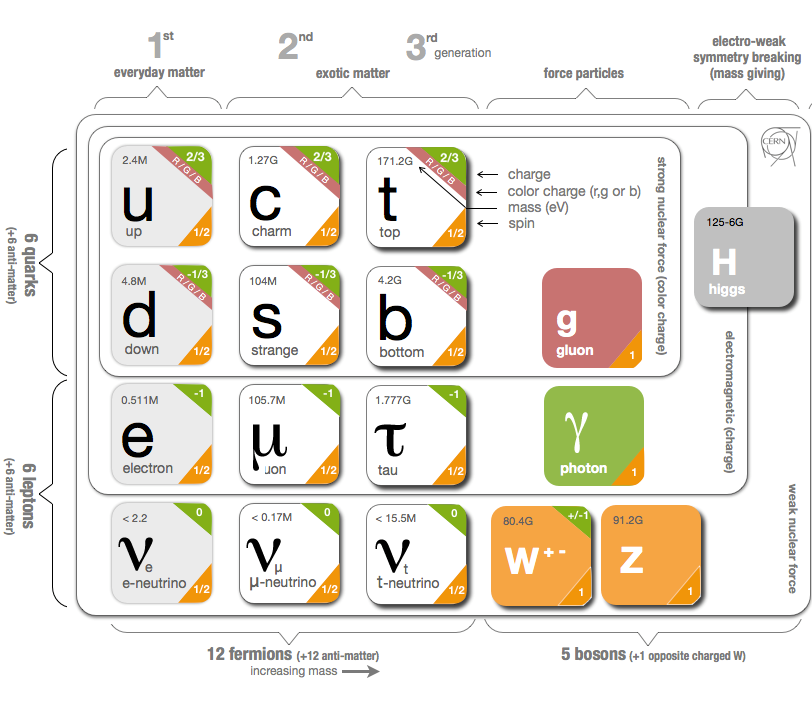
\includegraphics[width=0.90\textwidth]{../figs/Intro/StandardModel.png}}
    \caption{Standard Model Particles and Interations}
    \label{fig:SMtable}
  \end{center}
\end{figure}


%Protons and neutrons are baryons.

%%The electromagnetic and weak interactions are discussed in more details in Sec. \ref{sec:Intro_Electroweak} with the Higgs mechanism explained in \ref{sec:Intro_Higgs} and the strong interactions are discussed in more details in Sec. \ref{sec:Intro_QCD}. In addition to these three interaction, there is the fourth fundamental interaction known: the gravity. The gravity is not included into the SM.


